\documentclass{tufte-handout}
\usepackage{amsmath}
\usepackage{graphicx}
\graphicspath{ {./img/} }
\title{AdaBoost for Face Detection}
\author{Andr\'es Ponce}

\begin{document}
\maketitle

\begin{abstract}
AdaBoost stands for \textbf{Ada}ptive \textbf{Boosting}, 
which builds a strong classifier from many individually weak
learners.
\end{abstract}

\section{AdaBoost}
AdaBoost is a method for face detection which uses many simple
classifiers. The weak learner makes a simple binary decision
for a single feature
\[h_{1}(x) \in \{-1, 1\} \textrm{ ... } h_{T}(x) \in \{-1, 1\}\]

For all the $T$ features, we have a simple classifier which makes a decision 
that's better than a random decision. Then, if we take a weighted sum of the 
simple classifiers, we can get a strong classifier.
\footnote{In this formula, the $\alpha$ value is the weight of the classifier.}
\[ H_{T}(x) = \textrm{sign}(\sum_{t=1}^{T}\alpha_{t}h_{t}(x))\]

\section{AdaBoost Process}
We first assume a uniform distribution and choose a classifier with a minimal 
weighted error. Then we increase the weight of the misclassified elements 
and thus make our decision for the next round.

Then we repeat the step, and choose the classifier with the minimal weighted error.
Since in the previous step we increased the weights of the misclassified points, this
will ``pull" the classifier line towards those elements. After the second iteration
we again increase the weights of the misclassified elements.

\begin{marginfigure}
	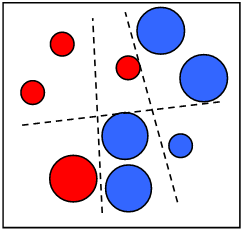
\includegraphics[scale=0.4]{adaboost}
	\caption{The three dashed lines are individually weak classifiers, since they all
	mislabel a couple of data points. However, if our model $H(x)$ uses all three classifers,
	the combined results will be quite strong.}
\end{marginfigure}

The main objective of AdaBoost is to find the model $h_{t}$ which classifies correctly 
at the highest rate. We also want to find the highest \textbf{margin} between the decision
boundary and the data points. We do this by using the negative exponent of $\alpha$.
\end{document}
